\subsubsection{Functional Principle} \label{section:license-google-functional}
\begin{itemize}
    \item test
\end{itemize}
Google's approach is based on a network service which allows to query the trusted Google Play license server in order to determine whether the user has a valid license.
The LVL is provided by Google in source code to be included in an App by the programmer. Thus its exact functionality and even structures and variable names can be studied by programmers. \cite{munteanLicense}
\newline
It has to be manually integrated into the application by the developer and allows a simple checking with Google and has a callback for the reply.
The developer can decide when and how often the application should check its license.
Upon initialization, the library connects to the Google Play Service which manages the connection between the device and the license server.
It sends a request for a license check to the server.
This is similar to \gls{drm}.
Adding the library to the application does not alter the function of the application, it just adds a call.
The developer only needs to handle the result of this call, as the library takes care of the complicated process, like the networking and web service, and returns the response of Google Play as soon as it arrives.
The developer is in full control of what happens with the response and whether access is granted.
Figure~\ref{fig:lvl} gives an overview how the parts are connected. \cite{digipomLvl} \cite{developersLicensingOverview}
\newline
\begin{figure}[h]
    \centering
    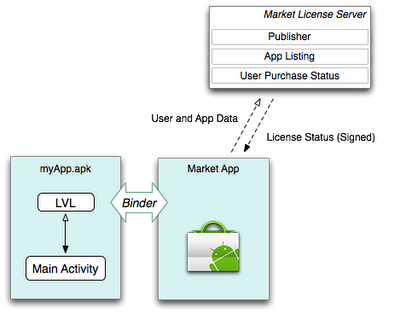
\includegraphics[width=0.8\textwidth]{data/lvl.png}
    \caption{Google's implementation of license checking \cite{developersLicensingOverview}}
    \label{fig:lvl}
\end{figure}
In order to start the validation process with the Google Server and determine the license status of the application, additional information has to be provided.
The \textit{LicenseChecker} has to be initiated with the package name of the application, a nonce, to ensure integrity of the response, as well as the callback for asynchronous handling, to start the call to the Play Service client.
The Google Play Service then adds the primary Google account username, the identity and other information and sends the license check request to the server.
On the Google Play server, it is checked whether the user has purchased the application and a corresponding response is send back to the Google Play Service, which returns it to the application. \cite{developersLicensingOverview}
\newline
The security of the response is very important.
It is achieved by public/private key encryption.
Each published application in the Play Store has a pair of keys.
The developer has to integrate the public key into the application, which is available in the Google Play developer console.
The private key is used to decrypt the communication with the server which encrypts its response with the private key.
This way it the origin of the response is ensured and tampering detected.
\cite{munteanLicense} \cite{developersLicensingOverview}
\newline
This mechanism requires an online connection to the internet, as it needs to connect to the Google server.
In case this is not possible, an internal error will be triggered which results in the license not being verified.
In addition, the Google Play Service has to be installed which comes preinstalled with the Google Apps, including the Google Play store.
It is a prerequisite to legally acquire an application with the \gls{lvl} since it is bought in the Play Store.
In case the application is installed and the Google Play Service is not installed, it cannot bind to it and thus cannot verify the license.
The developer can decide when and how often the license check should be done as well as whether the result should be stored for future requests or when no internet connection is available. \cite{developersLicensingAdding } \cite{developersLicensingOverview}
\newline
The \gls{lvl} mechanism replaces the old copy protection, which is no longer supported.
This license verification model can be enforced on all devices which have access to Google Play. \cite{developersLicensingAdding} \cite{developersLicensingOverview}
